\section{Genetic Effects}
\label{sec:genetic-effects}

Section to show the results of the Ed PGI $\to$ Education, labour earnings.
Clearly define the estimands, and then the estimating equations.


Write $D_i$ for education years, and $D_i(z')$ the potential outcome for Ed PGI value $z'$.

Write $Y_i$ for resulting labour market income, and $Y_i(z',d')$ the associated potential outcome for Ed PGI value $z'$ and education years $d'$.


Assumptions,
\[ Z_i^\text{\textcolor{red}{Random}} \indep D_i(.), Y_i(.,.) \]
and
\[ Z_i^\text{\textcolor{red}{Random}}
    \text{ is a good instrument for }
    Z_i^\text{\textcolor{ForestGreen}{Child}} \]

This gives identification for the effects of the Ed PGI on education years and labour market income,
\[ \partialdiff{z'} \E{D_i(z')}, \text{ and } \partialdiff{z'} \E{Y_i(z', D_i(z'))}. \]
Note that this is standard; the random component is strong instrument by design (a formula instrument), and everyone is a complier --- though the OLS estimate gives more weights to those with higher $Z_i^\text{\textcolor{red}{Random}}$ values.

\subsection{Genetic Results}

This will require using the random components as obviously related instruments for the other PGIs, respectively.

These results will likely be larger than in other papers, because of the measurement error reducing precision in previous work.




\begin{figure}[h!]
    \centering
    \singlespacing
    \caption{TODO: Make this show the binscatter of Ed PGI $\to$ Ed years, and income.  Regular colour line for the raw correlation, and yellow line for the random component.}
    \begin{subfigure}[b]{0.495\textwidth}
        \centering
        \caption{Earnings.}
        %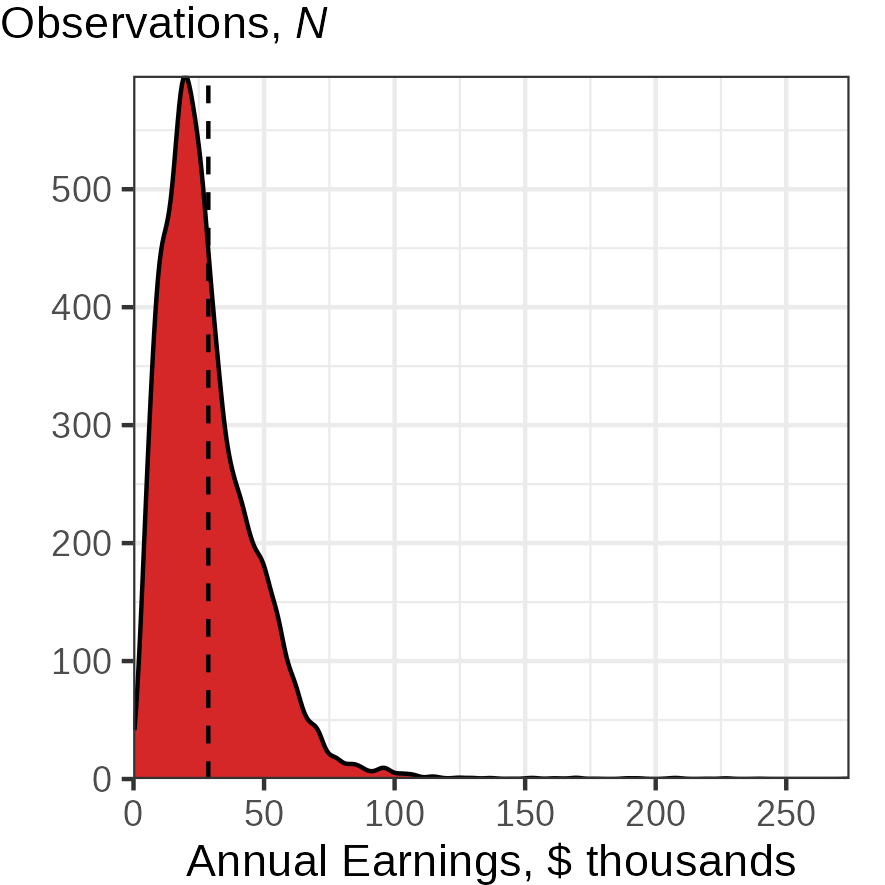
\includegraphics[width=\textwidth]{sections/figures/earnings-hist.png}
        \label{fig:earnings-hist}
    \end{subfigure}
    \begin{subfigure}[b]{0.495\textwidth}
        \centering
        \caption{Ed PGI $+$ Earnings.}
        %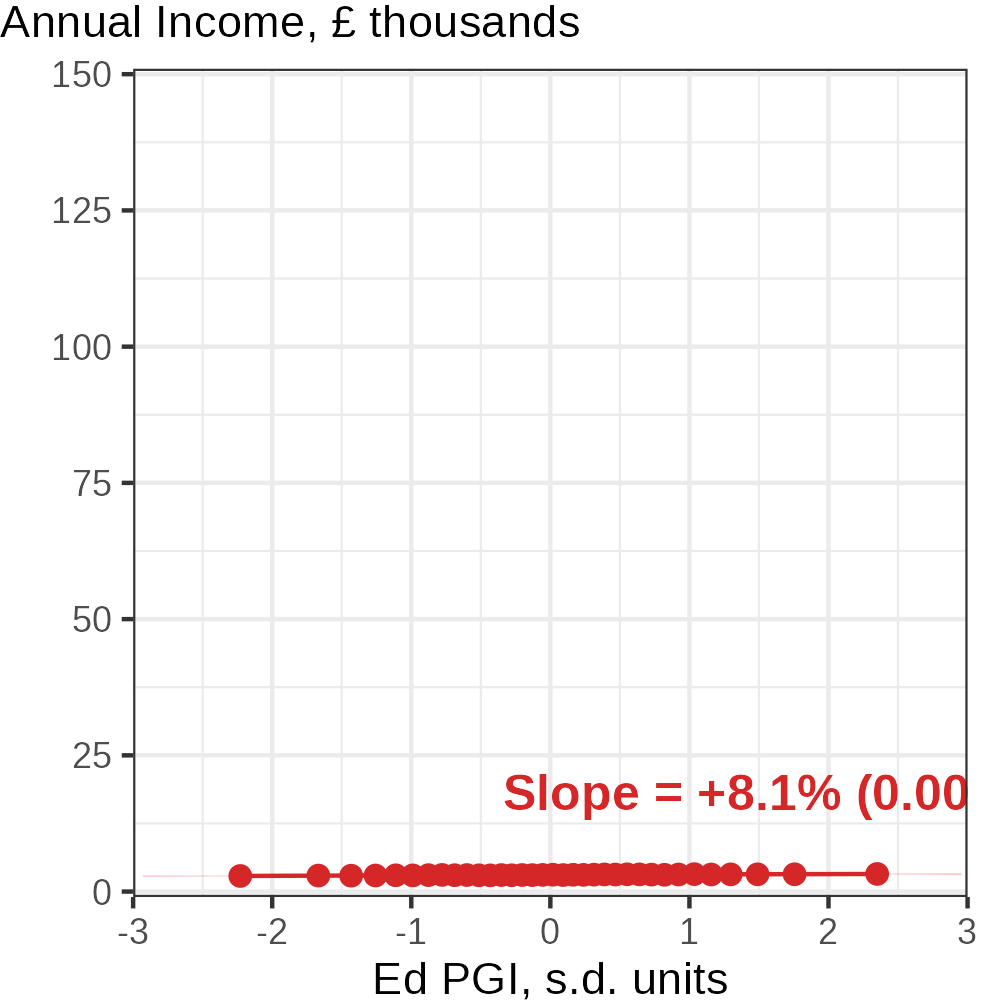
\includegraphics[width=\textwidth]{sections/figures/edpgi-earnings.png}
        \label{fig:edpgi-earnings}
    \end{subfigure}
    \label{fig:ukb-edpgi-earnings}
    \vspace{-1cm}
    \justify
    \footnotesize
    \textbf{Note}:
    This figure shows the marginal distribution of Ed PGI and education years among UKB household heads, in the analysis sample defined above.
    Ed PGI is normalised within-in sample by the UKB to have mean 0, and standard deviation 1; the distribution shape is unaffected by the normalisation --- i.e., it is roughly normally distributed regardless.
    3.4\% of the analysis sample reports education years less than 10 years (not included in panel b).
\end{figure}



\textbf{TODO:} a LaTeX table summarising the results, too.
